\section{Resultados y análisis}

A continuación se muestran las potencias calculadas a partir de los datos experimentales para cada montaje. 
\subsection{Generador Termoeléctrico}

A partir de los datos medidos (temperatura y voltajes) se obtienen las potencias, aplicada $P_A$, de carga $P_L$ y disipada por la resistencia interna $P_{R_i}$. Además, se interpolan los valores de $P_{open}$ usando una regresión de los datos suministrados. Estos datos se tomaron usando una escala de temperatura con precisión de décimas de grado y un rango de diferencia de temperatura  $\Delta T = 0 - 40 \si{\celsius}$. Estos valores se muestran en la figura \ref{fig:gen_powers}. Se observa que los datos de $P_A$ tienen un comportamiento escalonado, esto debido a que al aplicar una diferencia de potencial a la resistencia de carga, se debía dejar transcurrir un tiempo hasta observar la temperatura máxima alcanzada por la resistencia de calentamiento, y en ese tiempo, por lo que se registraron varios datos para un mismo voltaje aplicado. De la gráfica \ref{fig:gen_powers} también se puede corroborar que los datos obtenidos para las demás potencias son menores a la potencia aplicada, corroborando que la energía útil en efecto es menor que la energía suministrada, en concordancia con la segunda ley.

\begin{figure}[ht]
    \centering
    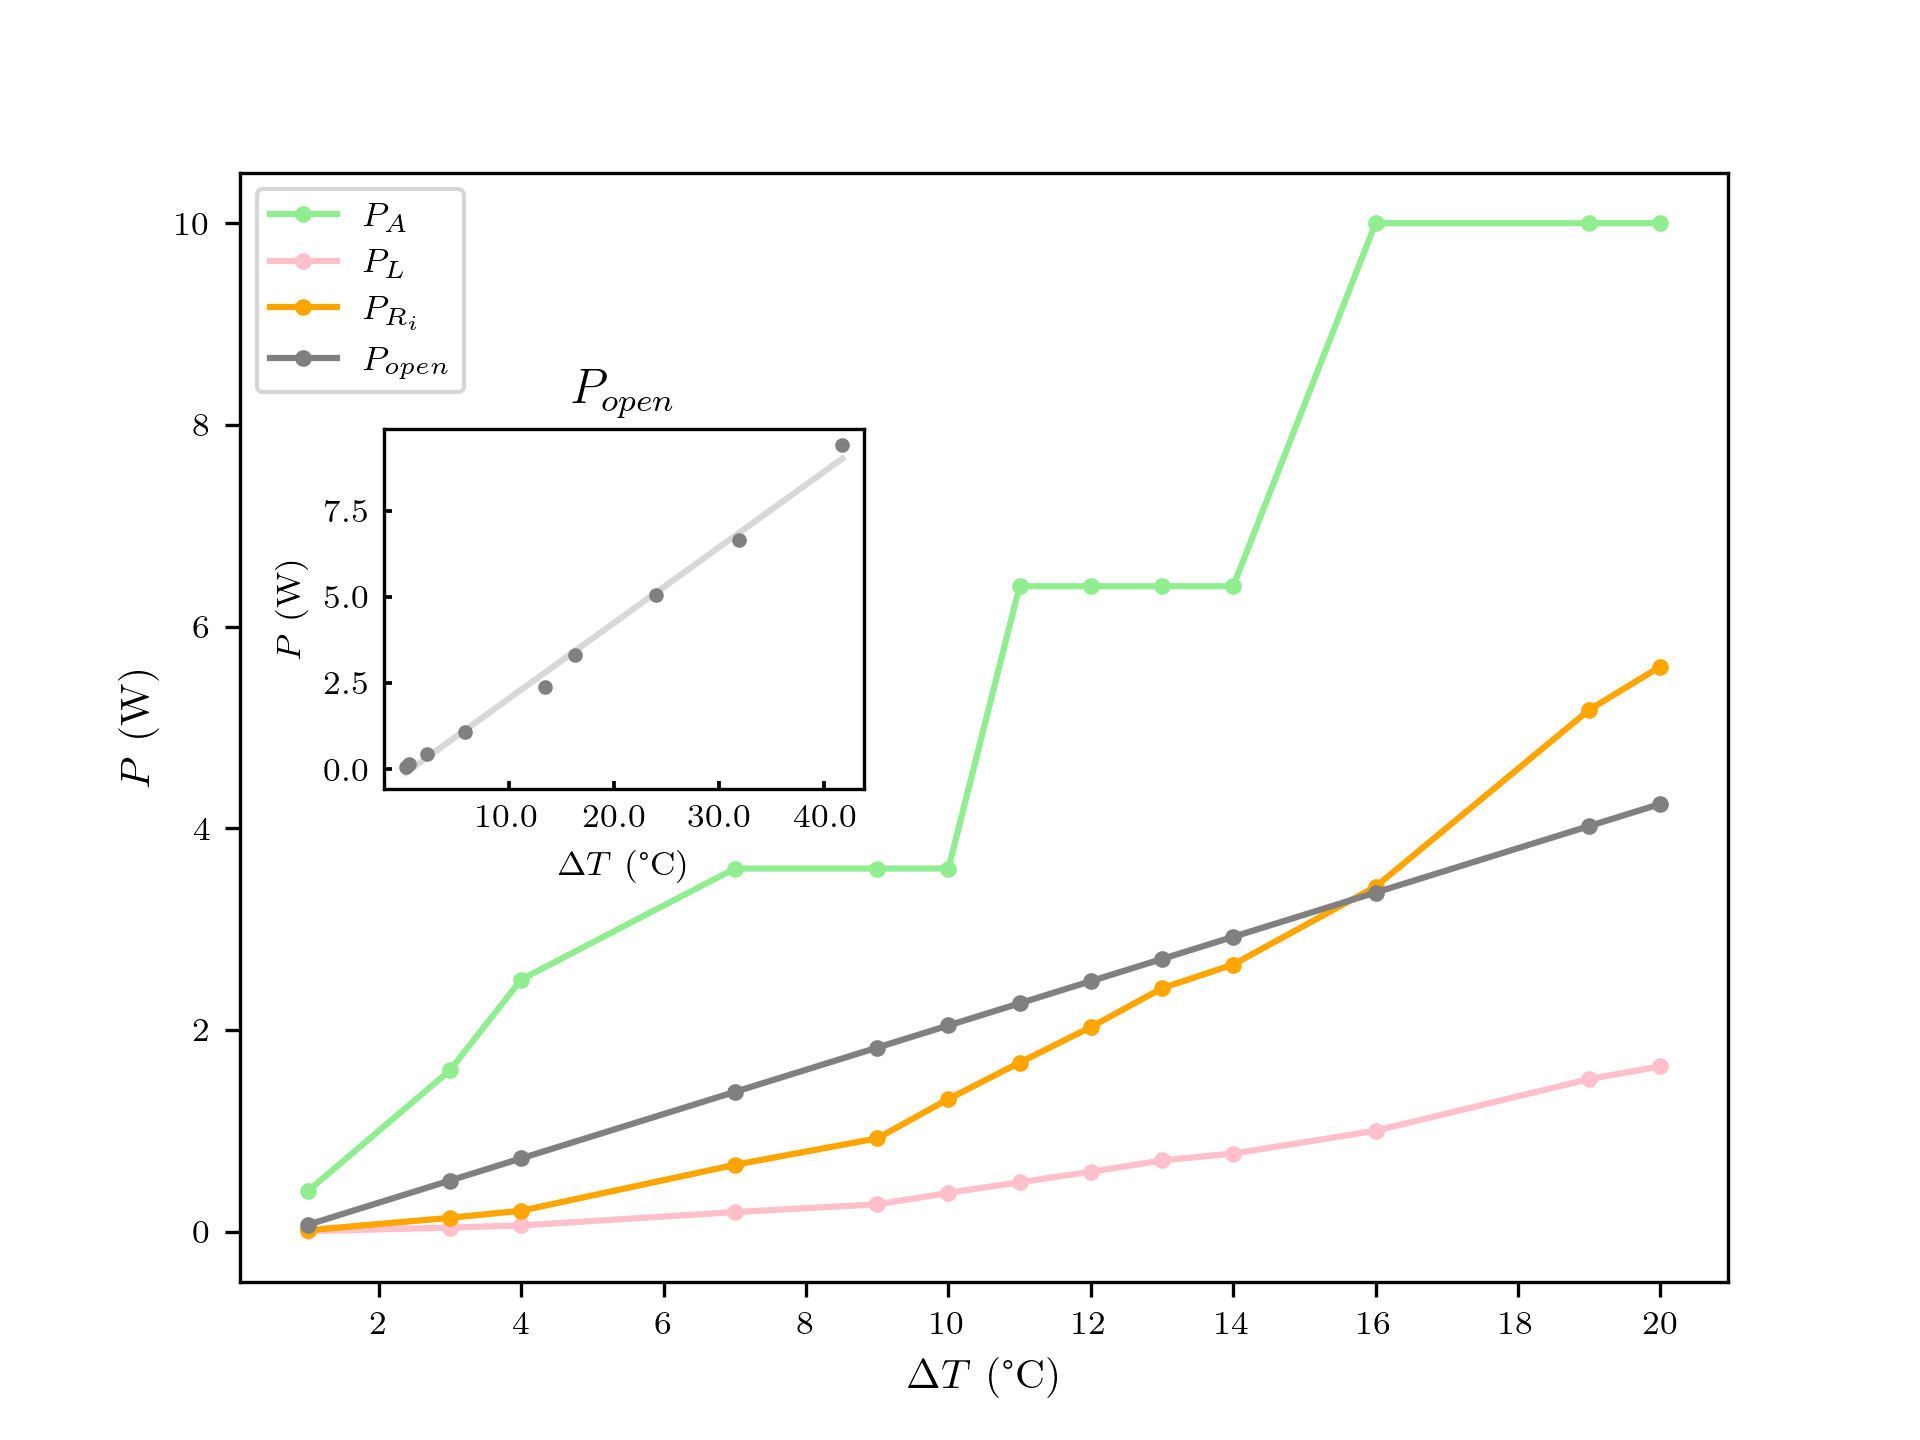
\includegraphics[width = 0.6\linewidth]{img/gen_powers.png}
    \caption{Potencias medidas para el módulo térmico usado como generador térmico. Los datos de $P_{open}$ se midieron en un rango distinto de temperatura y con una escala más fina (décimas de grado).}
    \label{fig:gen_powers}
\end{figure}

Ahora, calculando las eficiencias (nominal, de carnot y corregidas) se obtienen lo mostrado en la figura \ref{fig:etas}. 

\begin{figure}[ht]
    \centering
    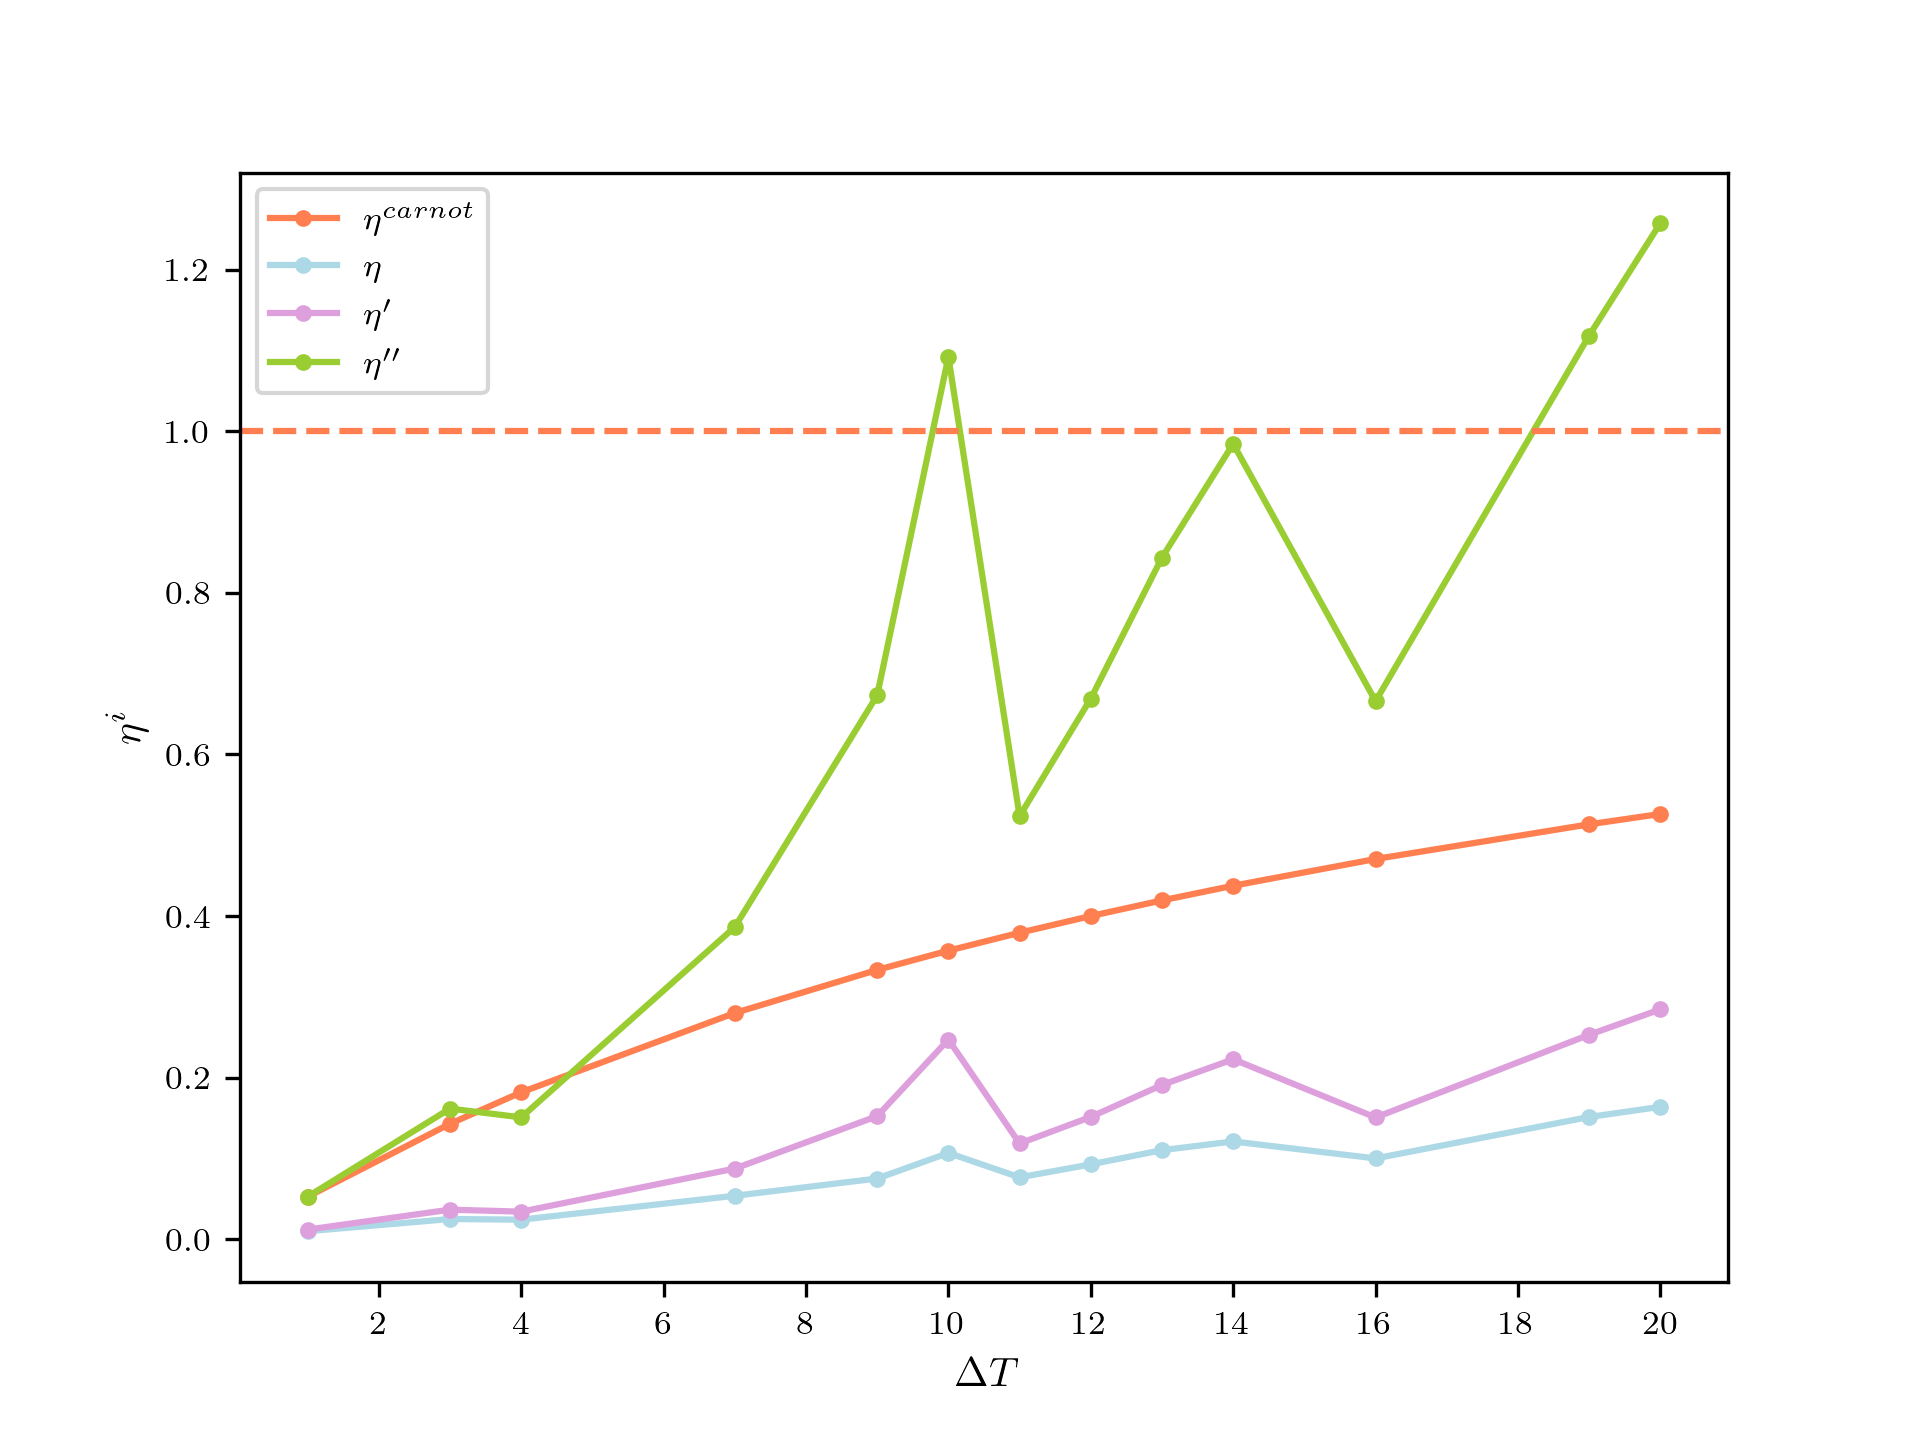
\includegraphics[width = 0.6\linewidth]{img/gen_etas.png}
    \caption{Comparación de las diferentes eficiencias calculadas como función de la diferencia de temperatura}
    \label{fig:etas}
\end{figure}

\subsection{Refrigerador}

De forma similar, se calculan las potencias involucradas en el montaje de refrigerador con el módulo Peltier. Se observa en la figura \ref{fig:refri_powers} naturalmente que se requiere una mayor cantidad de energía para lograr una diferencia de temperatura cada vez menor. 

\begin{figure}[ht]
    \centering
    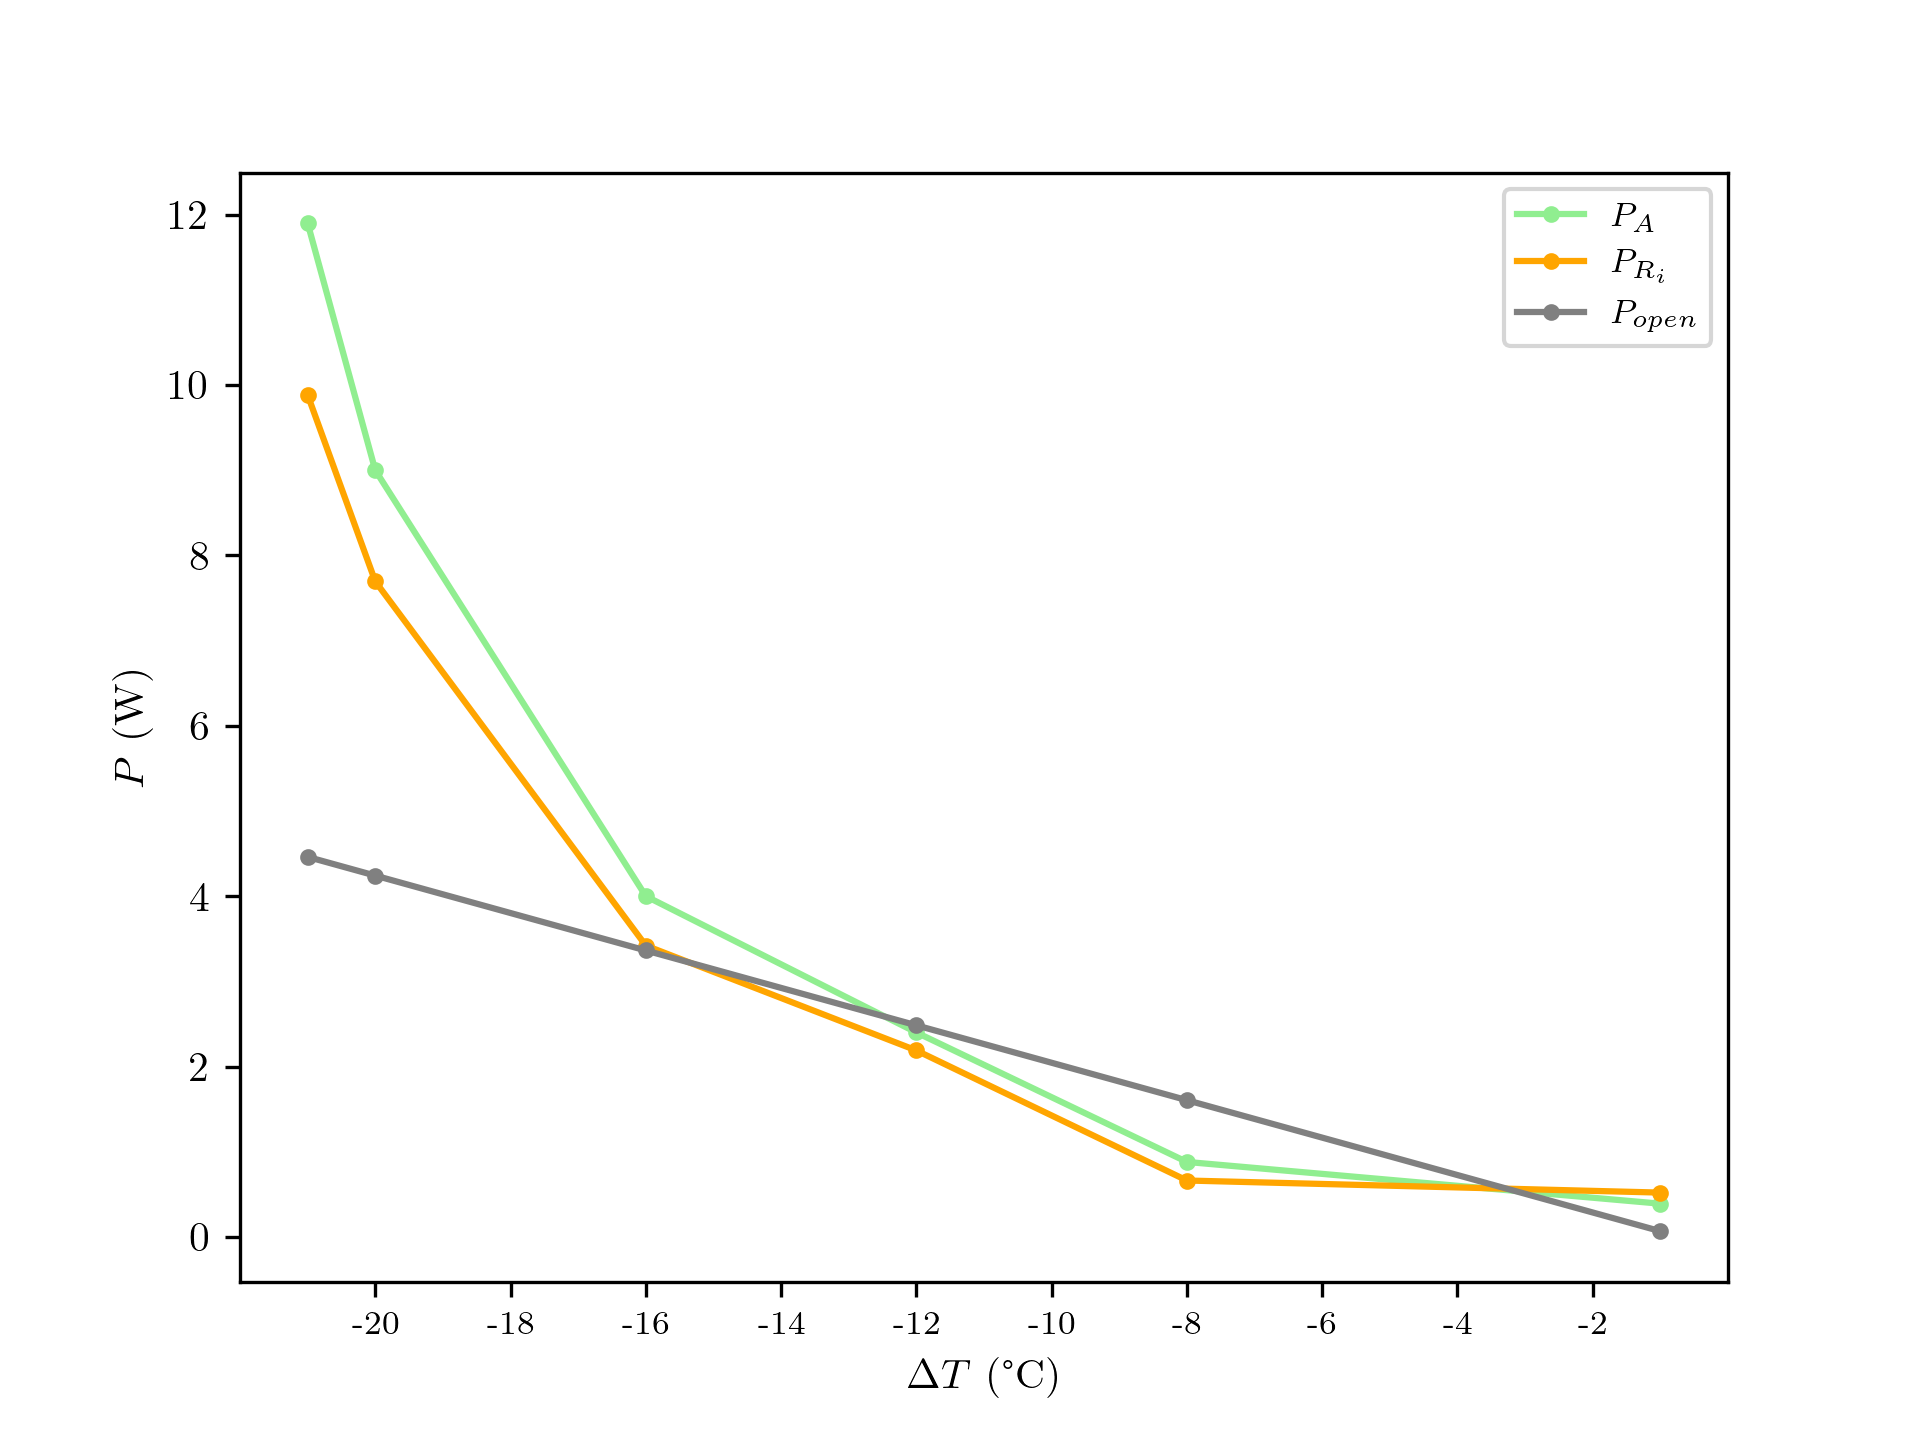
\includegraphics[width = 0.5\linewidth]{img/refri_powers.png}
    \caption{Potencias medidas para el módulo térmico usado como refrigerador. Se usa la misma recta de $P_{open}$ usada en el montaje anterior.}
    \label{fig:refri_powers}
\end{figure}

En la figura \ref{fig:refri_cops} se muestran los coeficientes de rendimiento $COP$ que se calcularon. Se observa que el valor ajustado $COP_{ad}$ sobrepasa el valor teórico. Nuevamente, este comportamiento se atribuye a una sobreestimación de la resistencia interna.

\begin{figure}[ht]
    \centering
    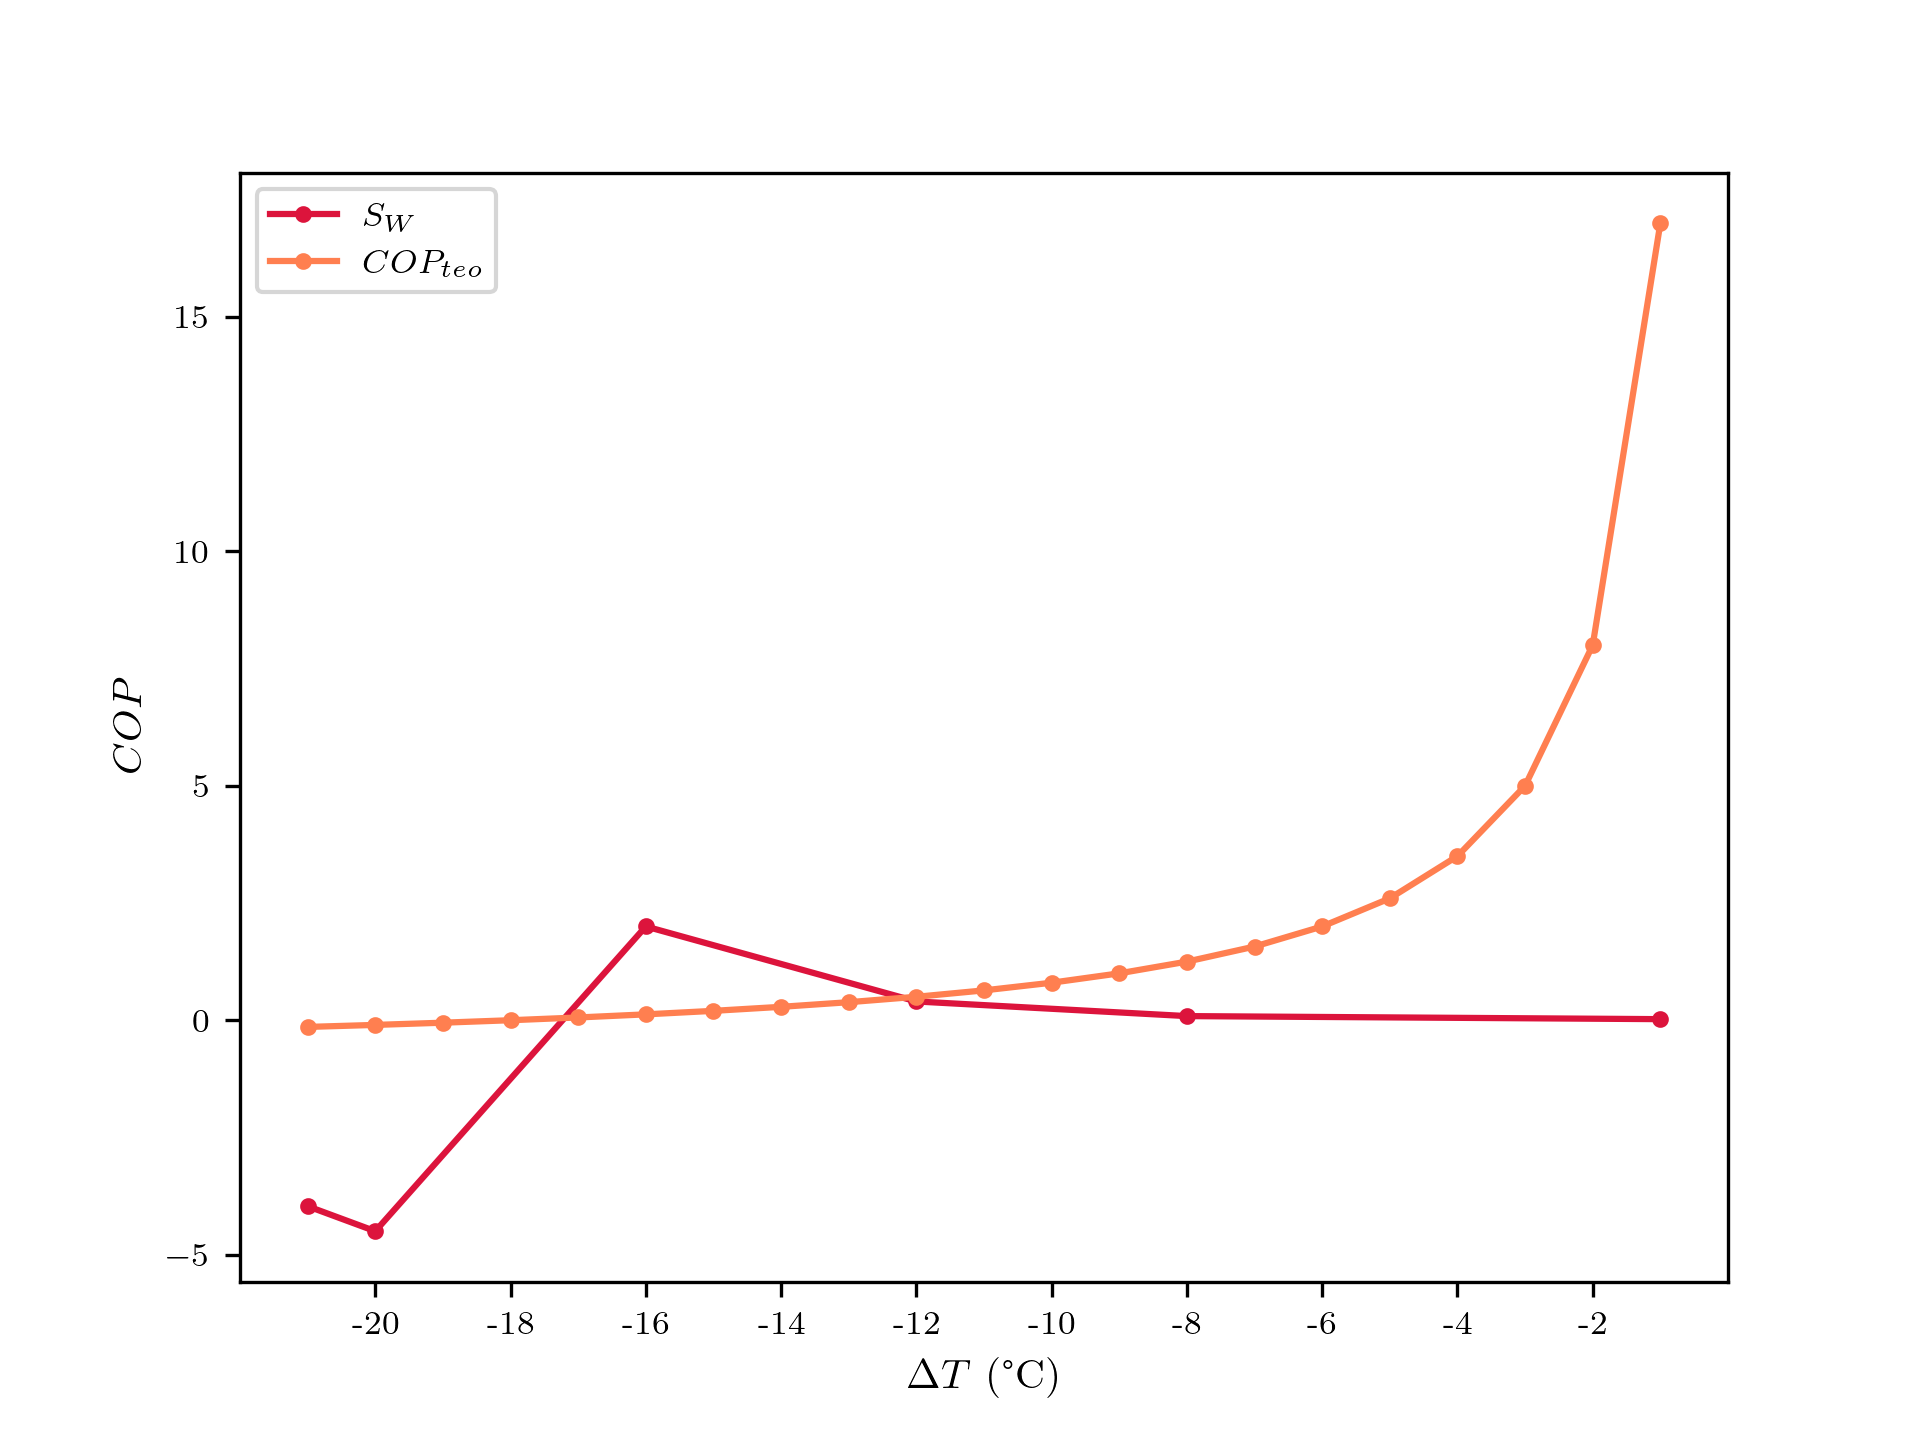
\includegraphics[width = 0.5\linewidth]{img/refri_cops.png}
    \caption{Comparación de los coeficientes de rendimiento.}
    \label{fig:refri_cops}
\end{figure}

\subsection{Ley de fourier para el módulo}

Sabiendo que el módulo está construido de 162 celdas de $\SI{6}{\milli\meter\squared}$ y que tiene un espesor de $\SI{2.5}{\milli\meter}$, se tiene que el coeficiente de conductividad térmica del módulo es $\SI{0.843}{\watt\per\meter\per\celsius}$

